\chapter{Parallel Computation for Audio and Image Processing}
\label{chap:fft}

Mathematical computations involving images can become quite intensive,
and thus parallel methods are of great interest.  Here we will be
primarily interested in methods involving {\bf Fourier} analysis.  

\section{General Principles}

\subsection{One-Dimensional Fourier Series}

A sound {\bf wave form} graphs volume of the sound against time.  Here,
for instance, is the wave form for a vibrating reed:\footnote{Reproduced
here by permission of Prof. Peter Hamburger, Indiana-Purdue University,
Fort Wayne. See http://www.ipfw.edu/math/Workshop/PBC.html }

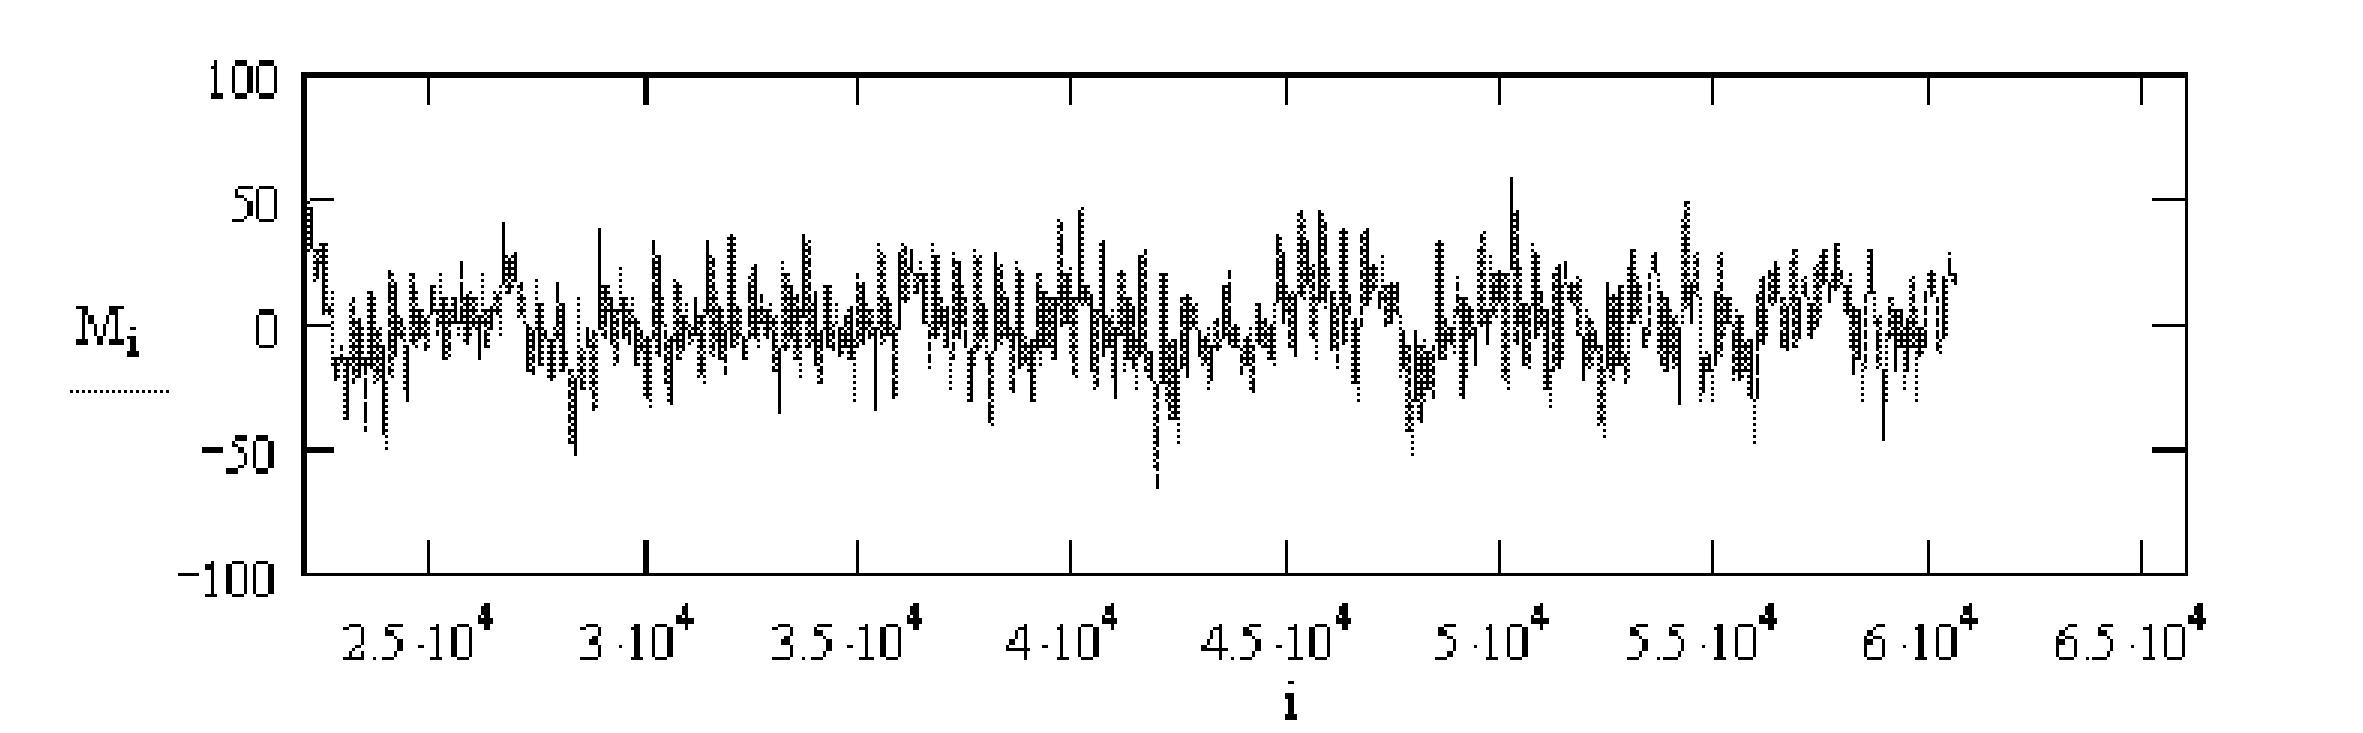
\includegraphics{Images/ReedTime.jpg}  

Recall that we say a function of time g(t) is \textbf{periodic}
(``repeating,'' in our casual wording above) with period T if if g(u+T)
= g(u) for all u. The \textbf{fundamental frequency} of g() is then
defined to be the number of periods per unit time,

\begin{equation}
f_{0}={1\over T}
\end{equation}

Recall also from calculus that we can write a function g(t) (not
necessarily periodic) as a Taylor series, which is an ``infinite
polynomial'':

\begin{equation}
\label{poly}
g(t)=\sum _{n=0}^{\infty }c_{n}t^{n}.
\end{equation}

The specific values of the $c_n$ may be derived by differentiating both
sides of (\ref{poly}) and evaluating at t = 0, yielding 

\begin{equation}
c_n = \frac{g^{(n)}(0)}{n!},
\end{equation}

where $g^{(j)}$ denotes the ith derivative of g().

For instance, for \( e^{t} \),

\begin{equation}
\label{exptaylor}
e^{t}=\sum _{n=0}^{\infty }\frac{1}{n!}t^{n}
\end{equation}

In the case of a repeating function, it is more convenient to use
another kind of series representation, an ``infinite trig polynomial,''
called  a {\bf Fourier series}.  This is just a fancy name for a
weighted sum of sines and cosines of different frequencies.  More
precisely, we can write any repeating function g(t) with period T and
fundamental frequency $f_0$ as    

\begin{equation} 
\label{f2t}
g(t)={\sum _{n=0}^{\infty }{a_{n}}\cos (2\pi nf_{0}t)}+{\sum _{n=1}^{\infty }{b_{n}}\sin (2\pi nf_{0}t)}
\end{equation}

for some set of weights $a_n$ and $b_n$.  Here, instead of having a
weighted sum of terms

\begin{equation}
1,\, \, t,\, \, t^{2},\, \, t^{3},\, \, ...
\end{equation}

as in a Taylor series, we have a weighted sum of terms

\begin{equation}
1,\, \, \cos (2\pi f_{0}t),\, \, \cos (4\pi f_{0}t),\, \, \cos (6\pi f_{0}t),\, \, ...
\end{equation}

and of similar sine terms. Note that the frequencies $nf_0$, in those
sines and cosines are integer multiples of the fundamental frequency of
x, $f_{0}$, called \textbf{harmonics}. 

The weights $a_n$ and $b_n$, n = 0, 1, 2, ... are called the
\textbf{frequency spectrum} of g().  The coefficients are calculated as
follows:\footnote{The get an idea as to how these formulas arise, see
Section \ref{vector}.  But for now, if you integrate both sides of
(\ref{f2t}), you will at least verify that the formulas below do work.}

\begin{equation}
\label{t2fi}
a_{0}=\frac{1}{T}\int _{0}^{T}g(t) ~ dt
\end{equation}

\begin{equation}
\label{t2fii}
a_{n}=\frac{2}{T}\int _{0}^{T}g(t) ~ cos(2\pi nf_{0}t) ~ dt
\end{equation}

\begin{equation}
\label{t2fiii}
b_{n}=\frac{2}{T}\int _{0}^{T}g(t) ~ sin(2\pi nf_{0}t) ~ dt
\end{equation}

By analyzing these weights, we can do things like machine-based voice
recognition (distinguishing one person's voice from another) and speech
recognition (determining what a person is saying).  If for example one
person's voice is higher-pitched than that of another, the first
person's weights will be concentrated more on the
higher-frequency sines and cosines than will the weights of the second.

Since g(t) is a graph of loudness against time, this representation of
the sound is called the {\bf time domain}.  When we find the Fourier
series of the sound, the set of weights $a_n$ and $b_n$ is said to be a
representation of the sound in the {\bf frequency domain}.  One can
recover the original time-domain representation from that of the
frequency domain, and vice versa, as seen in Equations (\ref{t2fi}),
(\ref{t2fii}), (\ref{t2fiii}) and (\ref{f2t}).  

In other words, the transformations between the two domains are inverses
of each other, and there is a one-to-one correspondence between them.
Every g() corresponds to a unique set of weights and vice versa.

Now here is the frequency-domain version of the reed sound:

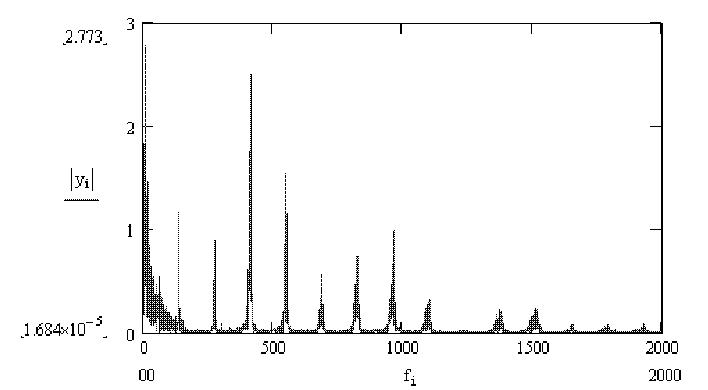
\includegraphics{Images/ReedFreq.jpg}

Note that this graph is very {}``spiky.{}'' In other words, even though
the reed's waveform includes all frequencies, most of the power of the
signal is at a few frequencies which arise from the physical properties
of the reed.   

Fourier series are often expressed in terms of complex numbers, making
use of the relation

\begin{equation}
e^{i \theta} = \cos(\theta) + i ~ \sin(\theta),
\end{equation}

where $i = \sqrt{-1}$.\footnote{There is basically no physical
interpretation of complex numbers.  Instead, they are just
mathematical abstractions.  However, they are highly useful
abstractions, with the complex form of Fourier series, beginning with
(\ref{compact}), being a case in point.

It is not assumed that you know complex variables well.  All that is
required is knowledge of how to add, subtract, multiply and divide, and
the definition of $|c|$ for complex c.}  

The complex form of (\ref{f2t}) is

\begin{equation}
\label{compact}
g(t) = \sum_{j = -\infty}^{\infty} c_j e^{2\pi i j \frac{t}{T}}.
\end{equation}

The $c_j$ are now generally complex numbers.  They are functions of the
$a_j$ and $b_j$, and thus form the frequency spectrum.

Equation (\ref{compact}) has a simpler, more compact form than
(\ref{f2t}).  Do you now see why I referred to Fourier series as trig
polynomials?  The series (\ref{compact}) involves the j$^{th}$ powers of
$e^{2\pi \frac{t}{T} }$.

\subsection{Two-Dimensional Fourier Series}

Let's now move from sounds to images.  Just as we were taking time to be a
continuous variable above, for the time being we are taking the position
within an image to be continuous too; this is equivalent to having
infinitely many pixels.  Here g() is a function of two variables,
g(u,v), where u and v are the horizontal and vertical coordinates of a
point in the image, with g(u,v) being the intensity of the image at that
point.  If it is a gray-scale image, the intensity is whiteness of the
image at that point, typically with 0 being pure black and 255 being
pure white.  If it is a color image, a typical graphics format is to
store three intensity values at a point, one for each of red, green and
blue.  The various colors come from combining three colors at various
intensities.

The terminology changes a bit.  Our original data is now referred to as
being in the {\bf spatial domain}, rather than the time domain. But the
Fourier series coefficients are still said to be in the frequency
domain.

\section{Discrete Fourier Transforms} 
\label{1dim}

In sound and image applications, we seldom if ever know the exact form
of the repeating function g().  All we have is a {\bf sampling} from
g(), i.e. we only have values of g(t) for a set of discrete values of t.

In the sound example above, a typical sampling rate is 8000 samples per
second.\footnote{See Section \ref{sampling} for the reasons behind
this.} So, we may have g(0), g(0.000125), g(0.000250), g(0.000375), and
so on.  In the image case, we sample the image pixel by pixel.

Integrals like (\ref{t2fi}) now change to sums.  

\subsection{One-Dimensional Data}
\label{onedimdft}

Let $X = (x_0,...,x_{n-1})$ denote the sampled values, i.e. the
time-domain representation of g() based on our sample data.  These are
interpreted as data from one period of g(), with the period being n and
the fundamental frequency being 1/n.  The frequency-domain
representation will also consist of n numbers, $c_0,...,c_{n-1}$,
defined as follows:

\begin{equation}
\label{dft}
c_k = 
\frac{1}{n} \sum_{j=0}^{n-1} x_j e^{-2\pi i jk/n} =
\frac{1}{n} \sum_{j=0}^{n-1} x_j q^{jk}
\end{equation}

where

\begin{equation}
q = e^{-2\pi i /n}
\end{equation}

again with $i = \sqrt{-1}$.  The array C of complex numbers $c_k$ is
called the {\bf discrete Fourier transform} (DFT) of X.
Note that (\ref{dft}) is basically a discrete analog of 
(\ref{t2fii}) and (\ref{t2fiii}).

Note that instead of having infinitely many frequencies, we only have n
of them, i.e. the n original data points $x_j$ map to n frequency weights
$c_k$.\footnote{Actually, in the case of $x_j$ real, which occurs with
sound data, we really get only n/2 frequencies.  The weight of the
frequences after k = n/2 turn out to be the {\bf conjugates} of those
before n/2, where the conjugate of a+bi is defined to be a-bi.}

The quantity q is a n$^{th}$ root of 1:

\begin{equation}
q^n = e^{-2 \pi i} = \cos(-2 \pi) + i \sin(-2 \pi) = 1
\end{equation}

Equation (\ref{dft}) can be written as

\begin{equation}
\label{CfromX}
C = \frac{1}{n} A X,
\end{equation}

where X is the vector $x_j$ and 

\begin{equation}
\label{vander}
A = 
\left (
\begin{array}{ccccc}
1 & 1 & 1 & ... & 1 \\
1 & q & q^2 & ... & q^{n-1} \\
... & ... & ... & ... & ... \\
1 & q^{n-1} & q^{2(n-1)} & ... & q^{(n-1)(n-1)}
\end{array}
\right )
\end{equation}

Here's R code to calculate A:

\begin{Verbatim}[fontsize=\relsize{-2},numbers=left]
makeamat <- function(n,u)  {
   m <- matrix(nrow=n,ncol=n)
   for (i in 1:n) {
      for (j in i:n) {
         if (i == j) {
            m[i,i] <- u^((i-1)^2)
         }
         else {
            m[i,j] <- u^((i-1)*(j-1))
            m[j,i] <- m[i,j]
         }
      }
   }
   m
}
\end{Verbatim}

\subsection{Inversion}

As in the continuous case, the DFT is a one-to-one transformation.  so
we can recover each domain from the other.  The details are important:

The matrix A in (\ref{vander}) is a special case of {\bf Vandermonde}
matrices, known to be invertible.  In fact, if we think of that matrix
as a function of q, A(q), then it turns out that

\begin{equation}
\label{vanderinv}
[A(q)]^{-1} = \frac{1}{n} A(\frac{1}{q})
\end{equation}

Thus (\ref{CfromX}) becomes

\begin{equation}
\label{XfromC}
X = n [A(q)]^{-1} C = A(\frac{1}{q}) C
\end{equation}

In nonmatrix terms:

\begin{equation}
\label{dftinv}
x_j = 
\sum_{k=0}^{n-1} c_k e^{2\pi ijk/n}  =
\sum_{k=0}^{n-1} c_k q^{-jk} 
\end{equation}

Equation (\ref{dftinv}) is basically a discrete analog of (\ref{f2t}).

\subsubsection{Alternate Formulation}

Equation (\ref{CfromX}) has a factor 1/n while (\ref{XfromC}) doesn't.
In order to achieve symmetry, some authors of material on DFT opt to
define the DFT and its inverse with $1/\sqrt{n}$ in (\ref{dft}) instead
of 1/n, and by adding a factor $1/\sqrt{n}$ in (\ref{dftinv}).  They
then include a factor $1/\sqrt{n}$ in (\ref{vander}), with the result
that $[A(q)]^{-1} = A(1/q)$.  Thus everything simplifies.  

Other formulations are possible.  For instance, the R {\bf fft()}
routine's documentation says it's ``unnormalized,'' meaning that
there is neither a $1/n$ nor a $1/\sqrt{n}$ in (\ref{dftinv}). 
When using a DFT routine, be sure to determine what it assumes about
these constant factors.

\subsection{Two-Dimensional Data}

The spectrum numbers $c_{rs}$ are double-subscripted, like the original
data $x_{uv}$, the latter being the pixel intensity in row u, column v
of the image, u = 0,1,...,n-1, v = 0,1,...,m-1.  Equation (\ref{dft})
becomes

\begin{equation}
\label{dft2} 
c_{rs} = \frac{1}{n} \frac{1}{m} 
\sum_{j=0}^{n-1} 
\sum_{k=0}^{m-1} 
x_{jk} e^{-2\pi i(\frac{jr}{n}+\frac{ks}{m})}
\end{equation}

where r = 0,1,...,n-1, s = 0,1,...,m-1.

Its inverse is

\begin{equation}
\label{dft2inv}
x_{rs} = 
\sum_{j=0}^{n-1}
\sum_{k=0}^{m-1}
c_{jk} e^{2\pi i(\frac{jr}{n}+\frac{ks}{m})}
\end{equation}

\section{Parallel Computation of Discrete Fourier Transforms}

\subsection{The Fast Fourier Transform}

Speedy computation of a discrete Fourier transform was developed
by Cooley and Tukey in their famous Fast Fourier Transform (FFT), which
takes a ``divide and conquer'' approach:

Equation (\ref{dft}) can be rewritten as

\begin{equation}
c_k = \frac{1}{n} \left [ 
\sum_{j=0}^{m-1} x_{2j} {q}^{2jk} +
\sum_{j=0}^{m-1} x_{2j+1} {q}^{(2j+1)k} ,
\right ] 
\end{equation}

where $m = n/2$. 

After some algebraic manipulation, this becomes

\begin{equation}
\label{recursive} 
c_k = \frac{1}{2} \left [ 
\frac{1}{m} \sum_{j=0}^{m-1} x_{2j} z^{jk} +
q^k \frac{1}{m} \sum_{j=0}^{m-1} x_{2j+1} z^{jk} 
\right ] 
\end{equation}

where $z = e^{-2\pi i/m}$.

A look at Equation (\ref{recursive}) shows that the two sums within the
brackets have the same form as Equation (\ref{dft}).  In other words,
Equation (\ref{recursive}) shows how we can compute an n-point FFT from
two $\frac{n}{2}$-point FFTs.  That means that a DFT can be computed
recursively, cutting the sample size in half at each recursive step. 

In a shared-memory setting such as OpenMP, we could implement this
recursive algorithm in the manners of Quicksort in Chapter
\ref{chap:sort}.  

In a message-passing setting, again because this is a divide-and-conquer
algorithm, we can use the pattern of Hyperquicksort, also in
Chapter \ref{chap:sort}.  

Some digital signal processing chips implement this in hardware, with a
special interconnection network to implement this algorithm.

\subsection{A Matrix Approach}

The matrix form of (\ref{dft}) is

\begin{equation}
\label{matrix}
C = \frac{1}{n} A X
\end{equation}

where A is n x n.  Element (j,k) of A is $q^{jk}$, while
element j of X is $x_j$.  This formulation of the problem then naturally
leads one to use parallel methods for matrix multiplication, as in 
Chapter \ref{chap:matrix}.

Divide-and-conquer tends not to work too well in shared-memory settings,
because after some point, fewer and fewer threads will have work to do.
Thus this matrix formulation is quite valuable.

\subsection{Parallelizing Computation of the Inverse Transform}  

The form of the DFT (\ref{dft}) and its inverse (\ref{dftinv}) are very
similar.  For example, the inverse transform is again of a matrix form
as in (\ref{matrix}); even the new matrix looks a lot like the old 
one.\footnote{In fact, one can obtain the new matrix easily from the
old, as explained in Section \ref{vector}.}

Thus the methods mentioned above, e.g. FFT and the matrix approach,
apply to calculation of the inverse transforms too.

\subsection{Parallelizing Computation of the Two-Dimensional Transform}
\label{par2d}

Regroup (\ref{dft2}) as:

\begin{eqnarray}
\label{dft2new}
c_{rs} &=& 
\frac{1}{n} 
\sum_{j=0}^{n-1}
\left (
\frac{1}{m}
\sum_{k=0}^{m-1}
x_{jk} e^{-2\pi i(\frac{ks}{m})}
\right )
e^{-2\pi i(\frac{jr}{n})} \\
&=&
\label{zzz}
\frac{1}{n}
\sum_{j=0}^{n-1}
y_{js}
e^{-2\pi i(\frac{jr}{n})}
\end{eqnarray}

Note that $y_{js}$, i.e. the expression between the large parentheses,
is the s$^{th}$ component of the DFT of the j$^{th}$ row of our data.
And hey, the last expression (\ref{zzz}) above is in the same form as
(\ref{dft})!  Of course, this means we are taking the DFT of the
spectral coefficients rather than observed data, but numbers are
numbers.  

In other words:  To get the two-dimensional DFT of our data, we first get
the one-dimensional DFTs of each row of the data, place these in rows,
and then find the DFTs of each column.  This property is called {\bf
separability}.

This certainly opens possibilities for parallelization.  Each thread
(shared memory case) or node (message passing case) could handle groups
of rows of the original data, and in the second stage each thread could
handle columns.

Or, we could interchange rows and columns in this process, i.e. put the
j sum inside and k sum outside in the above derivation.

\section{Available FFT Software}

\subsection{R}
\label{rfft}

As of now, R only offers serial computation, through its function {\bf
fft()}.  It works on both one- and two-dimensional (or more) data.  If
its argument {\bf inverse} is set to TRUE, it will find the inverse.

Parallel computation of a two-dimensional transform can be easily
accomplished by using {\bf fft()} together with the approach in Section
\ref{par2d} and one of the packages for parallel R in Chapter
\ref{chap:r}.  Here's how to do it in {\bf snow}:

\begin{lstlisting}[numbers=left]
parfft2 <- function(cls,m) {
   tmp <- parApply(cls,m,1,fft)
   parApply(cls,tmp,1,fft)
}
\end{lstlisting}

Recall that when {\bf parApply()} is called with a vector-valued
function argument, the output from row i of the input matrix is placed
in {\it column} i of the output matrix.  Thus in the second call above,
we used rows (argument 1) instead of columns.

\subsection{CUFFT}

Remember that CUDA includes some excellent FFT routines, in CUFFT.

\subsection{FFTW}

FFTW (``Fastest Fourier Transform in the West'') is available for free
download at \url{http://www.fftw.org}.  It includes versions callable from
OpenMP and MPI.

\section{Applications to Image Processing}

In image processing, there are a number of different operations which we
wish to perform.  We will consider two of them here.

\subsection{Smoothing}
\label{smoothing}

An image may be too ``rough.''  There may be some pixels which are
noise, accidental values that don't fit smoothly with the neighboring
points in the image.

One way to smooth things out would be to replace each pixel intensity
value\footnote{Remember, there may be three intensity values per pixel,
for red, green and blue.} by the mean or median among the pixels
neighbors.  These could be the four immediate neighbors if just a little
smoothing is needed, or we could go further out for a higher amount of
smoothing.  There are many variants of this.

But another way would be to apply a {\bf low-pass filter} to the DFT of
our image.  This means that after we compute the DFT, we simply delete
the higher harmonics, i.e.  set $c_{rs}$ to 0 for the larger values of r
and s.  We then take the inverse transform back to the spatial domain.
Remember, the sine and cosine functions of higher harmonics are
``wigglier,'' so you can see that all this will have the effect 
of removing some of the wiggliness in our image---exactly what we
wanted.

We can control the amount of smoothing by the number of harmonics we
remove.

The term {\it low-pass filter} obviously alludes to the fact that the
low frequencies ``pass'' through the filter but the high frequencies are
blocked.  Since we've removed the high-oscillatory components, the
effect is a smoother image.\footnote{Note that we may do more smoothing
in some parts of the image than in others.}

To do smoothing in parallel, if we just average neighbors, this is
easily parallelized.  If we try a low-pass filter, then we use the
parallelization methods shown here earlier.

\subsection{Example:  Audio Smoothing in R}

Below is code to do smoothing on sound.  It inputs a sound sequence {\bf
snd}, and performs low-pass filtering, setting to 0 all DFT terms having
{\it k} greater than {\tt maxidx} in (\ref{dft}).

\begin{Verbatim}[fontsize=\relsize{-2},numbers=left]
p <- function(snd,maxidx) {
   four <- fft(snd)
   n <- length(four)
   newfour <- c(four[1:maxidx],rep(0,n-maxidx))
   return(Re(fft(newfour,inverse=T)/n))
}
\end{Verbatim}

Here the {\bf Re()} function extracts the real part of a complex number.

\subsection{Edge Detection}

In computer vision applications, we need to have a machine-automated way
to deduce which pixels in an image form an edge of an object.

Again, edge-detection can be done in primitive ways.  Since an edge
is a place in the image in which there is a sharp change in the
intensities at the pixels, we can calculate slopes of the intensities, in
the horizontal and vertical directions.  (This is really calculating the
approximate values of the partial derivatives in those directions.)

But the Fourier approach would be to apply a high-pass filter.  Since an
edge is a set of pixels which are abruptly different from their
neighbors, we want to keep the high-frequency components and block out
the low ones.  

Again, this means first taking the Fourier transform of the original,
then deleting the low-frequency terms, then taking the inverse transform
to go back to the spatial domain.

Below we have ``before and after'' pictures, first of original data 
and then the picture after an edge-detection process has been
applied.\footnote{These pictures are courtesy of Bill Green of
the Robotics Laboratory at Drexel University.  In this case he is
using a Sobel process instead of Fourier analysis, but the result would
have been similar for the latter.  See his Web tutorial at
\url{www.pages.drexel.edu/~weg22/edge.html}, including the original
pictures, which may not show up well in our printed book here.}

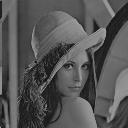
\includegraphics{Images/LENAG.jpg}  

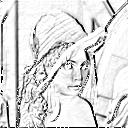
\includegraphics{Images/EDGESOB.jpg}  

The second picture looks like a charcoal sketch!  But it was derived
mathematically from the original picture, using edge-detection methods.

Note that edge detection methods also may be used to determine where
sounds (``ah,'' ``ee'') begin and end in speech-recognition applications.  
In the image case, edge detection is useful for face recognition, etc.

Parallelization here is similar to that of the smoothing case.

\section{R Access to Sound and Image Files}

In order to apply these transformations to sound and image files, you
need to extract the actual data from the files.  The formats are usually
pretty complex.  You can do this easily using the R {\bf tuneR} and {\bf
pixmap} libraries.

After extracting the data, you can apply the transformations, then
transform back to the time/spatial domain, and replace the data
component of the original class.

\section{Keeping the Pixel Intensities in the Proper Range}

Normally pixel intensities are stored as integers between 0 and 255,
inclusive.  With many of the operations mentioned above, both
Fourier-based and otherwise, we can get negative intensity values, or
values higher than 255.  We may wish to discard the negative values and
scale down the positive ones so that most or all are smaller than 256.

Furthermore, even if most or all of our values are in the range 0 to
255, they may be near 0, i.e. too faint.  If so, we may wish to multiply
them by a constant.

\section{Does the Function g() Really Have to Be Repeating?}

It is clear that in the case of a vibrating reed, our loudness function
g(t) really is periodic.  What about other cases?

A graph of your voice would look ``locally periodic."  One difference
would be that the graph would exhibit more change through time as you
make various sounds in speaking, compared to the one repeating sound for
the reed.  Even in this case, though, your voice {\it is} repeating
within short time intervals, each interval corresponding to a different
sound.  If you say the word {\it eye}, for instance, you make an ``ah''
sound and then an ``ee'' sound.  The graph of your voice would show one
repeating pattern during the time you are saying ``ah,'' and another
repeating pattern during the time you are saying ``ee.''  So, even for
voices, we do have repeating patterns over short time intervals.

On the other hand, in the image case, the function may be nearly
constant for long distances (horizontally or vertically), so a local
periodicity argument doesn't seem to work there.

The fact is, though, that it really doesn't matter in the applications
we are considering here.  Even though mathematically our work here has
tacitly assumed that our image is duplicated infinitely times
(horizontally and vertically),\footnote{And in the case of the cosine
transform, implicitly we are assuming that the image flips itself on
every adjacent copy of the image, first right-side up, then upside-own,
then right-side up again, etc.} we don't care about this.  We just want
to get a measure of ``wiggliness,'' and fitting linear combinations of
trig functions does this for us.

\section{Vector Space Issues (optional section)} 
\label{vector}

The theory of Fourier series (and of other similar transforms), relies
on vector spaces.  It actually is helpful to look at some of that here.
Let's first discuss the derivation of (\ref{dft}).  

Define X and C as in Section \ref{1dim}.  X's components are real, but
it is also a member of the vector space V of all n-component arrays of
complex numbers.  

For any complex number a+bi, define its {\bf conjugate},
$\overline{a+bi} = a-bi$.  Note that

\begin{equation}
\overline{e^{i \theta}} = \cos \theta - i \sin \theta = 
= \cos (-\theta) + i \sin (-\theta) =
e^{-i \theta} 
\end{equation}

Define an inner product (``dot product''),

\begin{equation}
[u,w] = \frac{1}{n} \sum_{j=0}^{n-1} u_j \bar{w}_j.
\end{equation}

Define

\begin{equation}
v_h = (1,q^{-h},q^{-2h}, ..., q^{-(n-1)h}), h = 0,1,...,n-1.
\end{equation}

Then it turns out that the $v_h$ form an orthonormal basis for
V.\footnote{Recall that this means that these vectors are orthogonal to
each other, and have length 1, and that they span V.} For example, to
show orthnogonality, observe that for $r \neq s$

\begin{eqnarray}
[v_r,v_s] &=& \frac{1}{n} \sum_{j=0}^{n-1} {v_r}_j \overline{v_s}_j \\
&=& \frac{1}{n} \sum_{j=0} q^{j(-r+s)} \\
&=& \frac{1-q^{(-r+s)n}}{n(1-q)} \\
&=& 0,
\end{eqnarray}

due to the identity  $1+y+y^2+....+y^k = \frac{1-y^{k+1}}{1-y}$ and the
fact that $q^n = 1$.  In the case r = s, the above computation shows
that $[v_r,v_s] = 1$.

The DFT of X, which we called C, can be considered the ``coordinates''
of X in V, relative to this orthonormal basis.  The kth coordinate is
then $[X,v_k]$, which by definition is (\ref{dft}).

The fact that we have an orthonormal basis for V here means that the
matrix A/n in (\ref{matrix}) is an orthogonal matrix.  For real numbers,
this means that this matrix's inverse is its transpose.  In the complex
case, instead of a straight transpose, we do a conjugate transpose,
$B = \overline{A/n}^t$, where t means transpose.  So, B is the inverse of
A/n.  In other words, in (\ref{matrix}), we can easily get back to X
from C, via

\begin{equation}
X = B C = \frac{1}{n} \bar{A}^t C.
\end{equation}

It's really the same for the nondiscrete case.  Here the vector space
consists of all the possible periodic functions g() (with reasonable
conditions placed regarding continuity etc.) forms the vector space, and
the sine and cosine functions form an orthonormal basis.  The $a_n$ and
$b_n$ are then the ``coordinates'' of g() when the latter is viewed as
an element of that space.  

\section{Bandwidth: How to Read the \textit{San Francisco Chronicle}
Business Page (optional section)}
\label{sampling}

The popular press, especially business or technical sections, often
uses the term \textbf{bandwidth}. What does this mean?

Any transmission medium has a natural range $[f_{min} \),\( f_{max}]$
of frequencies that it can handle well. For example, an ordinary
voice-grade telephone line can do a good job of transmitting signals of
frequencies in the range 0 Hz to 4000 Hz, where ``Hz'' means cycles
per second. Signals of frequencies outside this range suffer fade in
strength, i.e are \textbf{attenuated}, as they pass through the phone
line.\footnote{And in fact will probably be deliberately filtered out.}

We call the frequency interval [0,4000] the \textbf{effective
bandwidth} (or just the \textbf{bandwidth}) of the phone line.

In addition to the bandwidth of a \textbf{medium}, we also speak of the
bandwidth of a \textbf{signal}. For instance, although your voice is a
mixture of many different frequencies, represented in the Fourier series
for your voice's waveform, the really low and really high frequency
components, outside the range [340,3400], have very low power, i.e.
their $a_{n}$ and $b_{n}$ coefficients are small. Most of the power of
your voice signal is in that range of frequencies, which we would call
the effective bandwidth of your voice waveform.  This is also the reason
why digitized speech is sampled at the rate of 8,000 samples per second.
A famous theorem, due to Nyquist, shows that the sampling rate should be
double the maximum frequency. Here the number 3,400 is ``rounded up'' to
4,000, and after doubling we get 8,000.

Obviously, in order for your voice to be heard well on the other end
of your phone connection, the bandwidth of the phone line must be
at least as broad as that of your voice signal, and that is the case.

However, the phone line's bandwidth is not much broader than that
of your voice signal. So, some of the frequencies in your voice will
fade out before they reach the other person, and thus some degree
of distortion will occur. It is common, for example, for the letter
`f' spoken on one end to be mis-heard as `s'on the other end. This
also explains why your voice sounds a little different on the phone
than in person. Still, most frequencies are reproduced well and phone
conversations work well.

We often use the term ``bandwidth'' to literally refer to width,
i.e. the width of the interval $[f_{min},f_{max}]$.

There is huge variation in bandwidth among transmission media. As we
have seen, phone lines have bandwidth intervals covering values on the
order of $10^{3}$.  For optical fibers, these numbers are more on the
order of $10^{15}$.  

The radio and TV frequency ranges are large also, which is why, for
example, we can have many AM radio stations in a given city.  The
AM frequency range is divided into subranges, called {\bf channels}.
The width of these channels is on the order of the 4000 we need for a
voice conversation.  That means that the transmitter at a station needs
to shift its content, which is something like in the [0,4000] range, to
its channel range.  It does that by multiplying its content times a sine
wave of frequency equal to the center of the channel.  If one applies a
few trig identities, one finds that the product signal falls into the
proper channel!

Accordingly, an optical fiber could also carry many simultaneous phone
conversations.

Bandwidth also determines how fast we can set digital bits. Think of
sending the sequence 10101010...  If we graph this over time, we get a
``squarewave'' shape.  Since it is repeating, it has a Fourier series.
What happends if we double the bit rate?  We get the same graph, only
horizontally compressed by a factor of two.  The effect of this on this
graph's Fourier series is that, for example, our former $a_3$ will now
be our new $a_6$, i.e. the $2 \pi \cdot 3 f_0$ frequency cosine wave
component of the graph now has the double the old frequency, i.e. is now
$2 \pi \cdot 6 f_0$.  That in turn means that the effective bandwidth of
our 10101010... signal has doubled too.

In other words:  To send high bit rates, we need media with large
bandwidths.


